\documentclass[article]{report}             % Type of document

\usepackage[utf8]{inputenc}    		 	    % Encoding
\usepackage[english]{babel}			        % Language
\usepackage{geometry}           			% Page margin
\usepackage{graphicx}           			% For images
\usepackage{newcent}            			% Font
\usepackage{color}              			% Colors
\usepackage{listings}           			% Lists
\usepackage[footnote, nolist]{acronym}	    % Acronyms
\usepackage[absolute, overlay]{textpos}	    % Text positioning
\usepackage[babel=true]{csquotes}

\usepackage{fancyhdr}          			 % We might have a need for them
\usepackage{float}
\usepackage{tabularx}

\usepackage{latexsym}
\usepackage{pdfpages}
\usepackage{tikz}
\usepackage{ifthen}
\usepackage{wrapfig}
\usepackage{textcomp}
\usepackage{multicol}

\usepackage{listings} % includes code

\lstset{
	tabsize=4,
	language=matlab,
        basicstyle=\scriptsize,
        %upquote=true,
        aboveskip={0.5\baselineskip},
        columns=fixed,
        showstringspaces=false,
        extendedchars=true,
        breaklines=true,
        basicstyle=\normalsize,
        prebreak = \raisebox{2ex}[2ex][2ex]{\ensuremath{\hookleftarrow}},
        showtabs=false,
        showspaces=false,
        showstringspaces=false,
        identifierstyle=\ttfamily,
        keywordstyle=\color[rgb]{0,0,1},
        commentstyle=\color[rgb]{0.133,0.545,0.133},
        stringstyle=\color[rgb]{0.627,0.126,0.941},
	language=Java
}

\setlength{\columnsep}{1cm}
\setlength{\TPHorizModule}{\paperwidth}	% Used for textblock
\setlength{\TPVertModule}{\paperheight}	% Used for textblock

\title {Oral Presentation 1}
\parskip = 0.25cm              % Summary options (spaces between lines)

% Margin
\geometry{tmargin=2.5cm, bmargin=1.5cm, lmargin=2.5cm, rmargin=2cm}

\definecolor{blue}{rgb}{0.13,0.29,0.46}
\definecolor{red}{rgb}{1,0,0}
\definecolor{couleur_titre}{rgb}{0.20, 0.45, 0.80}
\definecolor{couleur_nom}{rgb}{0.11, 0.6, 0.18}

\renewcommand{\labelitemi}{$\bullet$}
\renewcommand{\contentsname}{Table of contents}

% Title at the top of the page
\pagestyle{fancyplain} \chead{}\lhead{\textit{Team Dedalus}} \rhead{\textcolor{couleur_titre}{\emph{\textit{Project: SkyLands}}}}

\title {Oral presentation 3}
\author {Romain\and Renaud\and Aenora\and Erwan}
\date {}

%
% Document
%
\begin{document}
	\thispagestyle{empty}
  	\begin{titlepage} 
		\vspace*{1cm} 
  		\begin{center} 
  			{\huge{\textsc{3rd Oral} \\ ~ \\{\large From}\\ ~\\ Team \\  ~ \\ }}
	  		\includegraphics[width = 14cm]{images/Titles/Dedalus.png}
			\\ ~ \\ ~ \\ ~ \\ ~ \\ ~ \\ ~ \\ ~ \\ ~ \\ ~ \\ ~ \\ ~ \\ ~ \\ ~ \\ ~ 
		\end{center}
  		\hfill {\large Romain \textsc{Biessy}}
  		\hfill {\large Renaud \textsc{Gaubert}}
  		\hfill {\large Aenora \textsc{Tye}}
  		\hfill {\large Erwan  \textsc{Vasseure}}
  	\end{titlepage} 

  	\tableofcontents
  		\pagenumbering{arabic}
  		\newpage
		
		\chapter{\textcolor{blue}{Introduction}}
			According to the string theory, there exist another universe where we sold millions of copy of this game! Unfortunatly, in this universe we though worked our hardest we still need some time.\\

			Implementing the Minecraft-like part of the game was the work we had to do for the last oral presentation and that was the easy part! For this presentation our goal was to implement the strategy part. At first it seemed easy, then we discovered the joy of programming an AI. Pathfinding and RTS were both a pain to implement. \\

 			Moreover, with the english major projects of Max and Fuji and the methodology's project, we had less time to work on the project. Also having our oral presentation on a monday didn't help. However we managed to have a pretty good result and to fix the bugs you saw on the previous presentation\\

 			On the other hand, our work was not only focused on the AI part, we also had fun implementing structures. The most impressing of them is what we named the dark tower and is present only in plain Islands, it took us about four whole days of coding to implement and can still be improved.\\
			
			We also had to deal with graphism problems such as the shadow managment which could not be completly implemented because of the fps drop it causes (it almost crash the game). The final part we had to deal with is the integration of the save and load functions to the menu which will be presented to you further in the report.\\
			
			To put it in a nutshell, we worked very hard for this oral presentation and have some amazing results which were not planned in the book of specifications. 
  		\chapter{\textcolor{blue}{PathFinding}}
			\section{A star 2d}
			\section{A star 3d}
				
		\chapter{\textcolor{blue}{Entities and actions}}
			\section{Robots}
				Since we needed enemies for our game, we decided to design it in a futurist style to match our game's story. We decided to go for the basic enemy of every science fiction story or game and created a robot mesh on Blender. The mesh model has simple shapes since our game itself is supposed to be "Minecraft-like" therefore cubic-shaped. As for the texture, they were implemented in-game and are also very simple black and white patterns.\\

Regarding the animations, we did them very simple too; there are only five different animations for death, turning around, shooting, slump and walking. Romain implemented the mesh textures and animations in the game afterwards.\\

However, we faced many problems with trying to export .blend 3D model to .mesh and tried with the 3DS-max software too. Implementing the animations wasn't a simple task either since the tool are too "old" and not always compatible with the current software we are using.
			\section{Shooting}
				We have two different shoot system for the AI and the player. The one for the AI is really simple whereas we wanted something more enjoyable for the player.
				\subsection{For the AI}
					At first for the AI, it will check every few seconds if it can shoot at an enemy. It simply cast a ray from its head to the adverse entity and then check if there are obstacles in between. We didn't want them to test this operation every frame for two reasons:\\
On the one hand to save some precious fps, as you can guess when there will be many AI on the field the fps will decrease a lot so we're already thinking of this matter.\\
On the other hand, this makes our AI looks more humans. Obviously we, poor little creatures, can't process all the information on the screen each frame. So we try to be fair, we don't want the AI to be invincible.

Once the AI know that someone is at range, it will simply create a mesh representing the bullet. This bullet will cast a new ray every few milliseconds to check if it is hitting something.
				\subsection{For the player}
					That's a bit different for the player. There is no more guns but fireballs. The player can hold the left mouse button down to create a fireball in front of him. It will grow while the button is pressed and will be thrown if the max size is reached or if the button is released.\\
Then this is quite the same than if this is a bullet. Of course the bigger the fireball is the more damage it will inflict.\\

Even thought this is a simple idea, we think it improves the gameplay. In a way it let more options to the player to choose how to kill the enemies.
		\chapter{\textcolor{blue}{The global AI}}
			There exist another kind of AI than the one for the entities. This is a global AI which is supposed to build buildings and give orders to its units. This is the actual enemy of the player.\\

Basically this AI want to destroy the base of the player and to weaken him. But here comes the issue of the difficulty. How to oppose to the player an adequate resistance ? Well the idea we found is simple. This AI bases its choice on the player's actions. 
		\chapter{\textcolor{blue}{Saving and Loading the game}}
			\section{Algorithm}
				The save and load algorithm of the terrain weren't modified since the last oral presentaion. As you know each different block possess an id (for example the id of the grass blocks is  1) which is stored in char whose weight is only one bite. Thus we can store the terrain in binary files fairly easily using the C\#'s native functions.\\
					
					We basically use a StreamWritter and a streamReader to save and load islands. However for this oral presentation, new things were added, such as robots and it did not suffice to only save the terrain, we had to save the entities.
					
					This time we choosed the easy way, registering the id of an entity and its position next to one another. Here is an explanatory diagram :\\						
							\begin{center}
								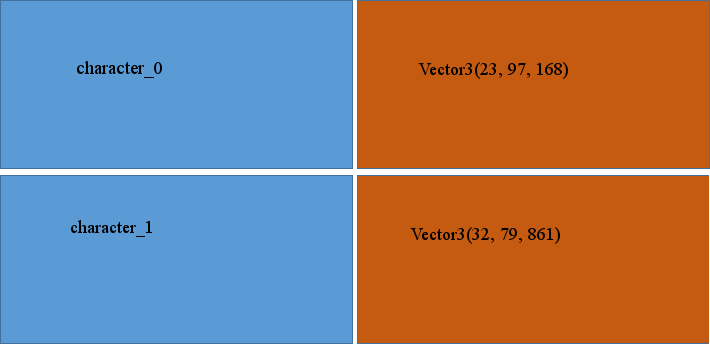
\includegraphics{images/Save.png}
							\end{center}
							
			\section{A new menu}
					With the save and load algorith, we felt that our old menu wasn't adapted to the mindset we had for this game. We didn't want the player to be able to choose what Island he could go on or what size! This menu was intended for debug purposes not for ou final product.\\

					So, in order to adapt the old menu to the mindset we thought of, we redesigned the buttons as well as the entire menu. Basically, we wanted a more futuristic menuand more dynamic.

			\section{Integration to the menu}
					As I've already said, the menu we had was intended for debug purposes only. Our idea for this menu was to let him create only one world and then to let him choose between 


		\chapter{\textcolor{blue}{Structures}}
			\section{Behind the scenes}
				Handling the structures was an easy task therefore, we decided to complexify it, making it easier to implement more than one structure at a time. The basic idea was to not just have multiple list of structures in the island class and then have a switch which would choose the list according to the biome.\\

				After thinking about a little bit we decided to make use of the inheritance via the abstract Biome class which implemented the methode populate calling the list of structure which is contained in every derived class of Biome.
				\begin{center}
					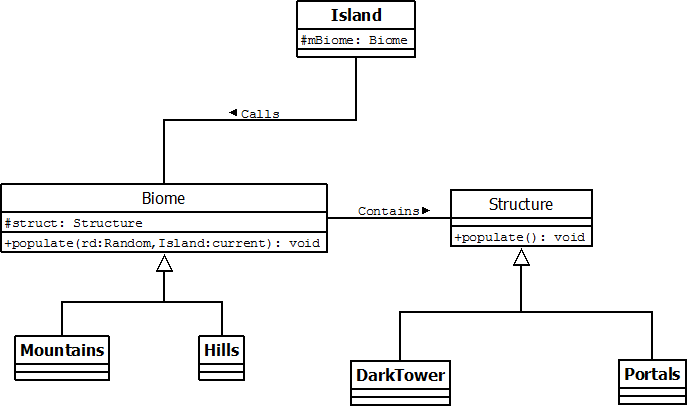
\includegraphics[width=15cm]{images/Structures.png}
				\end{center}

			\section{Portals}
			\section{Buildings}
			\section{Generating the base and placing it on the map}

		\chapter{\textcolor{blue}{The dark tower}}
			\section{The main building}
			\section{The floors}
			\section{Bridges}
			\section{Lower towers}
		\chapter{\textcolor{blue}{Graphics}}
			\section{Shadows}
			\section{Real shadows}
			\section{Creating the meshes}
		
		\chapter{\textcolor{blue}{Conclusion}}
			Unfortunately you have reached the end of this marvelous report! As you've seen throughout this report, we have worked very hard for this oral presentation. The result talk for themselves and the goal fixed were reached.\\
			
			Most of the game is still a work in progress (WIP), much has to be done in little time. However, the team is still standing and ready to work on those things !
			
			
\end{document}